\section{Yao's Protocol}
\label{sec:protocol}

This section provides a complete description of Yao's \emph{garbled circuits protocol} and how the protocol incorporates \ac{OT}.  Though the protocol described here was first published by Goldreich, Micali, and Wigderson\cite{goldreich1987play}, the terminology used in this section follows more recent publications\cite{hazay2010efficient}. In all cases though the concepts are similar and there is a direct mapping between the two.

The protocol is presented here twice, first in a less formal format that includes some reasoning for each step in the protocol, and a second time, fully describing each step taken by both parties. The former description is intended to make the latter one easier to follow.

\begin{algorithm}[H]
    \floatname{algorithm}{Protocol}
    \caption{Yao's Garbled Circuits Protocol}
    \label{alg:yao}
    \begin{algorithmic}[1]
        \STATE \ac{P1} generates a boolean circuit representation $c_c$ of \ac{f} that takes input $i_{P1}$ from \ac{P1} and $i_{P2}$ from \ac{P2}.
        \STATE \ac{P1} transforms $c_c$ by garbling each gate's computation table, creating garbled circuit $c_g$.
        \STATE \ac{P1} sends both $c_g$ and the values for the input wires in $c_g$ corresponding to $i_{P1}$ to \ac{P2}.
        \STATE \ac{P2} uses \emph{1-out-of-2 \ac{OT}} to receive from \ac{P1} the garbled values for $i_{P2}$ in $c_g$.
        \STATE \ac{P2} calculates $c_g$ with the garbled versions of $i_{P1}$ and $i_{P2}$ and outputs the result.
    \end{algorithmic}
\end{algorithm}

\subsection{Intuitive Description of the Protocol}

This section attempts to provide a high level explanation of how Yao's protocol works, as well as some of the reasoning behind its construction. It is included to make the following detailed description of the protocol easier to follow.

\ac{P1} and \ac{P2} wish to compute function \emph{f} securely, so that their inputs to the function remain secret. They begin doing so by modeling \emph{f} as a boolean circuit. \ac{P1} then ``garbles'' the circuit by replacing all boolean values in the circuit with pseudo-random looking strings, and then keeping this mapping secret.  This is done for the input and output wires of every gate in the circuit, with the exception of the circuits output gates; the values of these gates' output wires are left un-garbled.

\ac{P1} then replaces each bit of his input with the pseudo-random string that maps to that bit's input on the corresponding input wire into circuit. \ac{P1} then sends the garbled circuit and his garbled input to \ac{P2}.

\ac{P2} receives both the garbled circuit and \ac{P1}'s garbled input. However, since all input wires into the circuit have been garbled and only \ac{P1} has the mapping between the garbled values and the underlying bits, \ac{P2} does not know what values to input into the circuit to match her input bits. In other words, for each input wire into the circuit, \ac{P2} can select one of two random strings to input (corresponding to 0 or 1), but does not know which of these correspond to her desired input bit.

In order to learn which pseudo-random string to select for each of \ac{P2}'s input wires, \ac{P2} engages in a \emph{1-out-of-2 \ac{OT}} with \ac{P1} for each bit of \ac{P2}'s input. For each round of the \ac{OT}, \ac{P2} submits the bit she wishes to learn, receives the corresponding string.  Note that the properties of \ac{OT} prevent \ac{P1} from learning about \ac{P2}'s input in this process.

Once \ac{P2} has received all of the strings corresponding to her input into the circuit, she holds everything needed to compute the output of the circuit: her garbled inputs, \ac{P1}'s garbled inputs, and the garbled circuit itself. Further, she has obtained these values without \ac{P1} learning her inputs, nor \ac{P2} learning \ac{P1}'s inputs.

\ac{P2} then begins to compute the circuit by entering the pseudo-random strings that correspond to each bit of her and \ac{P1}'s input into the corresponding input wire and using the resulting garbled output string as an input to the next gate. \ac{P2} may try to learn information about \ac{P1}'s inputs by watching the execution of the circuit. The protocol prevents \ac{P2} from doing so though the manner that each computation table for each gate was constructed.

Recall that the computation table for every gate in the circuit was constructed so that each pair of inputs produces a output string that represents the correct boolean result, but which appears pseudo-random to \ac{P2}.  In other words, instead of mapping from $\{0, 1\} \times \{0, 1\} \to \{0, 1\}$, all gates in the circuit become a function mapping two random looking strings to another uniformly distributed pseudo-random string, or $f(\{0, 1\}^{|k|}, \{0, 1\}^{|k|}) \to \{0, 1\}^{|k|}$, where $|k|$ is the size of the value returned by the hash function. Since \ac{P2} never learns the mapping between strings used in the table and their underlying boolean values, \ac{P2} learns nothing by watching the outputs of each gate.

Recall that the values returned by the output gates in the circuit are not obscured. This results in \ac{P2} learning the value of $f(i_{P1}, i_{P2})$ once the computation has finished.  \ac{P2} then completes the protocol by sharing this computed value with \ac{P1}.


\subsection{Detailed Description of the Protocol}

This section provides a more precise explanation of each step of Yao's protocol, specifying how each step of the is carried out by both parties.  The numbering of subsections here followings the numbering used in protocol \ref{alg:yao}.


\subsubsection{Generating A Boolean Circuit Representation of the Function}

Before it can be securely evaluated, the function \emph{f} must be converted into an equivalent boolean circuit $c$ so that $\forall x, y \rightarrow f(x, y) = c(x, y)$. The strategies for optimally doing so may be function specific, and are beyond the scope of the protocol.  For the purposes of this paper though, it is sufficient to note that there exists a mapping from any polynomial time function with fixed sized inputs to a boolean circuit that calculates the same output\cite{goldreich1987play}.


\subsubsection{Garbling Truth Tables}

Once \ac{P1} has constructed a boolean circuit representation $c$ of $f$, the next step is to garble the truth table for each gate in $c$, generating a garbled version of the circuit, $c_g$ (ie $c \to c_g$).

\begin{figure}[t]
    \centering
    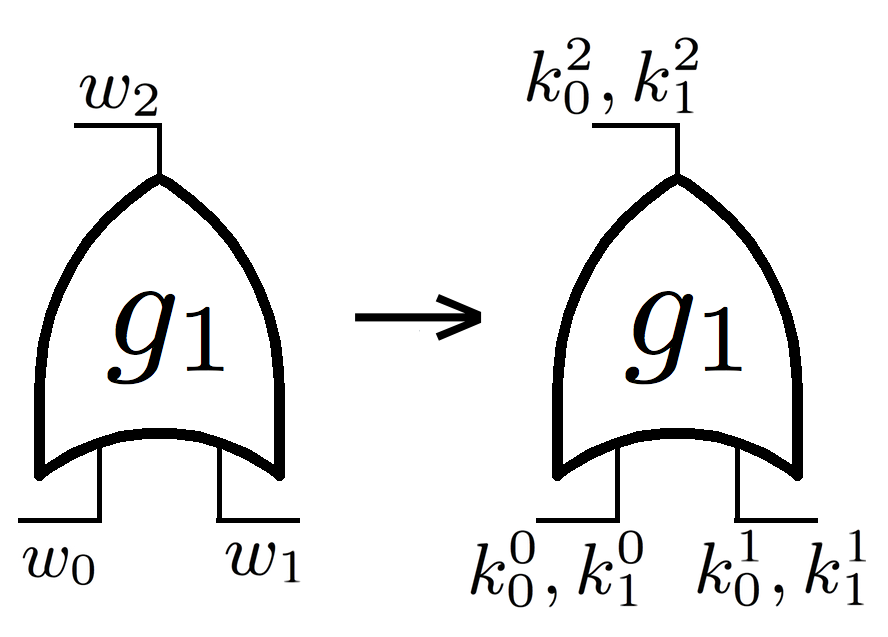
\includegraphics[width=\columnwidth]{images/or_gate}
    \caption{Garbling a single gate}
    \label{fig:garblegateimg}

    \subfloat[Original Values]{
        \begin{tabular}{ c | c || c }
            \hline
            $w_0$ & $w_1$ & $w_2$ \\
            \hline
            0 & 0 & 0 \\
            \hline
            0 & 1 & 1 \\
            \hline
            1 & 0 & 1 \\
            \hline
            1 & 1 & 1 \\
            \hline
        \end{tabular}
        \label{fig:gategarblepre}
    }
    \subfloat[Garbled Values]{
        \begin{tabular}{ c | c || c || c }
            \hline
            $w_0$ & $w_1$ & $w_2$ & garbled value \\
            \hline
            $k^0_0$ & $k^0_1$ & $k^0_2$ & $H(k^0_0 || k^0_1 || g_1) \oplus k^0_2$\\
            \hline
            $k^0_0$ & $k^1_1$ & $k^1_2$ & $H(k^0_0 || k^1_1 || g_1) \oplus k^1_2$\\
            \hline
            $k^1_0$ & $k^0_1$ & $k^1_2$ & $H(k^1_0 || k^0_1 || g_1) \oplus k^1_2$\\
            \hline
            $k^1_0$ & $k^1_1$ & $k^1_2$ & $H(k^1_0 || k^1_1 || g_1) \oplus k^1_2$\\
            \hline
        \end{tabular}
        \label{fig:gategarblepost}
    }
    \caption{Computation table for $g^{OR}_1$}
    \label{fig:gategarble}
\end{figure}

\begin{figure}[t!]
    \centering
    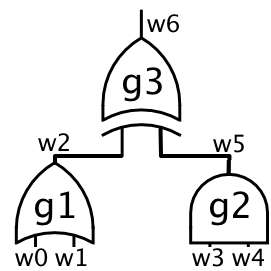
\includegraphics[width=\columnwidth]{images/multi_gates}
    \caption{Composing several gates into a Simple Circuit}
    \label{fig:garblecircuitimg}
    \subfloat[Original Values]{
        \begin{tabular}{ c | c || c }
            \hline
            $w_3$ & $w_4$ & $w_5$ \\
            \hline
            0 & 0 & 0 \\
            \hline
            0 & 1 & 0 \\
            \hline
            1 & 0 & 0 \\
            \hline
            1 & 1 & 1 \\
            \hline
        \end{tabular}
        \label{fig:andgatepre}
    }
    \subfloat[Garbled Values]{
        \begin{tabular}{ c | c || c || c }
            \hline
            $w_3$ & $w_4$ & $w_5$ & garbled value \\
            \hline
            $k^0_3$ & $k^0_4$ & $k^0_5$ & $H(k^0_3 || k^0_4 || g_2) \oplus k^0_5$\\
            \hline
            $k^0_3$ & $k^1_4$ & $k^0_5$ & $H(k^0_3 || k^1_4 || g_2) \oplus k^0_5$\\
            \hline
            $k^1_3$ & $k^0_4$ & $k^0_5$ & $H(k^1_3 || k^0_4 || g_2) \oplus k^0_5$\\
            \hline
            $k^1_3$ & $k^1_4$ & $k^1_5$ & $H(k^1_3 || k^1_4 || g_2) \oplus k^1_5$\\
            \hline
        \end{tabular}
        \label{fig:andgatepost}
    }
    \caption{Computation table for $g^{AND}_2$}
    \label{fig:andgate}

    \subfloat[Original Values]{
        \begin{tabular}{ c | c || c }
            \hline
            $w_2$ & $w_5$ & $w_6$ \\
            \hline
            0 & 0 & 0 \\
            \hline
            0 & 1 & 1 \\
            \hline
            1 & 0 & 1 \\
            \hline
            1 & 1 & 0 \\
            \hline
        \end{tabular}
        \label{fig:xorgatepre}
    }
    \subfloat[Garbled Values]{
        \begin{tabular}{ c | c || c || c }
            \hline
            $w_2$ & $w_5$ & $w_6$ & garbled value \\
            \hline
            $k^0_2$ & $k^0_5$ & $k^0_6$ & $H(k^0_2 || k^0_5 || g_3) \oplus k^0_6$\\
            \hline
            $k^0_2$ & $k^1_5$ & $k^1_6$ & $H(k^0_2 || k^1_5 || g_3) \oplus k^1_6$\\
            \hline
            $k^1_2$ & $k^0_5$ & $k^1_6$ & $H(k^1_2 || k^0_5 || g_3) \oplus k^1_6$\\
            \hline
            $k^1_2$ & $k^1_5$ & $k^0_6$ & $H(k^1_2 || k^1_5 || g_3) \oplus k^0_6$\\
            \hline
        \end{tabular}
        \label{fig:xorgatepost}
    }
    \caption{Computation table for $g^{XOR}_3$}
    \label{fig:xorgate}
\end{figure}

To see how \ac{P1} does this, first consider a single logical OR gate, $g^{OR}_1$, represented in figure \ref{fig:garblegateimg}. Initially \ac{P1} generates the values for this gate as normal, resulting in the truth table in figure \ref{fig:gategarblepre}. \ac{P1} then generates a key for each possible value for each wire in the gate.  This results in 6 keys being generated, one for each of the two possible boolean values on each of the three wires in the gate.

\ac{P1} then encrypts each entry in the table for the output wire using the keys used for the corresponding inputs.  The gate identifier serves as a nonce and is only included in this construction to ensure that the same values are never encrypted twice in the circuit.  \ac{P1} then randomly orders the rows the table, further obscuring the underlying boolean values\footnote{To simplify the presentation, this step is not shown in figure \ref{fig:garblegateimg}.}).

This encryption plays two important roles in the protocol.  First, since the output of each encryption operation is assumed be random (i.e. the hash function is assumed to perform like a random oracle), it removes any correlation between the underlying truth values in the table and the resulting garbled values. Even though this gate produces three identical boolean values, the garbled values all uniformly distributed, revealing nothing about the underlying value being encrypted.

Second, encrypting the output keys under the input keys prevents \ac{P2}, the circuit evaluator, from playing with the circuit and considering other inputs other than those provided by \ac{P1}. \ac{P2} can only obtain one of the output keys from the table, since she will only have, at most, the necessary input keys to the gate to decrypt one value for the output wire.

Once \ac{P1} has garbled the values for one gate, he can continue the process to compose an arbitrarily large circuit.  Figure \ref{fig:xorgate} shows how multiple garbled gates can be composed together into a simple circuit, and the how the keys from each gate are carried forward into the next gate, blinding the computing party from the learning the intermediate values being calculated.

The only gates in the circuit that do not need to be garbled are the output gates, or gates who's wires do not serve as input wires to another gate.  The values from these gates can remain unobscured since they are outputting the final result of the circuit, a value which \ac{P2} is allowed to learn.


\subsubsection{Sending Garbled Values to \ac{P2}}

Once \ac{P1} has finished generating the garbled circuit, he then needs to garble his input to the function, creating a mapping of $i_{P1}$ to its garbled equivalents.  \ac{P1} begins this process by replacing the first bit of his input with the corresponding key for that input wire in the circuit.  For example, \ac{P1}'s first bit was input into $w_0$, and the value of $i^0_{P1}$ was 1, \ac{P1} would select $k^1_0$ to be the first value in his input to the garbled circuit. \ac{P1} then repeats this procedure for the remaining bits in his input, creating \ac{P1}'s garbled input. \ac{P1} then sends the garbled circuit $c_g$ and his garbled input to \ac{P2}.

\subsubsection{Receiving \ac{P2}'s Input Values through \ac{OT}}

\ac{P2} receives $c_g$ and \ac{P1}'s garbled input, but still needs the garbled representation of her own input to compute the circuit. Recall that \ac{P1} has the garbled values for all of \ac{P2}'s input wires, but has no knowledge of what values correspond to \ac{P2}'s true input. \ac{P2}, inversely, knows the bits of her own input, but not the corresponding keys for her input wires in $c_g$.

\ac{P2} maps the first bit of her input to its corresponding garbled value by engaging in \emph{1-out-of-2 \ac{OT}}s with \ac{P1}, where \ac{P1}'s inputs are $(k^0_1, k^1_1)$, and \ac{P2}'s input is 0 or 1, depending on the first bit of \ac{P2}'s input.  \ac{P2} performs additional \ac{OT}s with \ac{P1} for all values $0 < i < |i_{P2}|$ to achieve her full garbled input into $c_g$.

\subsubsection{Computing the Garbled Circuit}

Once \ac{P2} has both garbled inputs and the garbled circuit, she can straight forwardly compute the circuit.  For each input gate, \ac{P2} looks up the corresponding value from \ac{P1} and \ac{P2}'s garbled input values and uses them as keys to decrypt the output value from the gate's garbled truth table.  Since \ac{P2} does not know which output key these two input keys correspond to, \ac{P2} must try to decrypt each of the four output keys.  If the protocol has been carried out correctly, only one of the four values will decrypt correctly.  The other three decryption attempts will produce $\bot$. The newly decrypted key then becomes an input key to the next gate.

\ac{P2} continues this process until she reaches the output wires of the circuit.  Each of these wires output a single, unencrypted bit.  \ac{P2} then reassembles the output bits and has the correct solution for the \ac{f} encoded by $c_g$.  \ac{P2} completes the protocol by sending the output of the circuit to \ac{P1}.
1) \oplus$
